% Options for packages loaded elsewhere
\PassOptionsToPackage{unicode}{hyperref}
\PassOptionsToPackage{hyphens}{url}
%
\documentclass[
]{article}
\usepackage{amsmath,amssymb}
\usepackage{lmodern}
\usepackage{iftex}
\ifPDFTeX
  \usepackage[T1]{fontenc}
  \usepackage[utf8]{inputenc}
  \usepackage{textcomp} % provide euro and other symbols
\else % if luatex or xetex
  \usepackage{unicode-math}
  \defaultfontfeatures{Scale=MatchLowercase}
  \defaultfontfeatures[\rmfamily]{Ligatures=TeX,Scale=1}
\fi
% Use upquote if available, for straight quotes in verbatim environments
\IfFileExists{upquote.sty}{\usepackage{upquote}}{}
\IfFileExists{microtype.sty}{% use microtype if available
  \usepackage[]{microtype}
  \UseMicrotypeSet[protrusion]{basicmath} % disable protrusion for tt fonts
}{}
\makeatletter
\@ifundefined{KOMAClassName}{% if non-KOMA class
  \IfFileExists{parskip.sty}{%
    \usepackage{parskip}
  }{% else
    \setlength{\parindent}{0pt}
    \setlength{\parskip}{6pt plus 2pt minus 1pt}}
}{% if KOMA class
  \KOMAoptions{parskip=half}}
\makeatother
\usepackage{xcolor}
\usepackage[left=3cm,right=3cm,top=2cm,bottom=2cm]{geometry}
\usepackage{color}
\usepackage{fancyvrb}
\newcommand{\VerbBar}{|}
\newcommand{\VERB}{\Verb[commandchars=\\\{\}]}
\DefineVerbatimEnvironment{Highlighting}{Verbatim}{commandchars=\\\{\}}
% Add ',fontsize=\small' for more characters per line
\usepackage{framed}
\definecolor{shadecolor}{RGB}{248,248,248}
\newenvironment{Shaded}{\begin{snugshade}}{\end{snugshade}}
\newcommand{\AlertTok}[1]{\textcolor[rgb]{0.94,0.16,0.16}{#1}}
\newcommand{\AnnotationTok}[1]{\textcolor[rgb]{0.56,0.35,0.01}{\textbf{\textit{#1}}}}
\newcommand{\AttributeTok}[1]{\textcolor[rgb]{0.77,0.63,0.00}{#1}}
\newcommand{\BaseNTok}[1]{\textcolor[rgb]{0.00,0.00,0.81}{#1}}
\newcommand{\BuiltInTok}[1]{#1}
\newcommand{\CharTok}[1]{\textcolor[rgb]{0.31,0.60,0.02}{#1}}
\newcommand{\CommentTok}[1]{\textcolor[rgb]{0.56,0.35,0.01}{\textit{#1}}}
\newcommand{\CommentVarTok}[1]{\textcolor[rgb]{0.56,0.35,0.01}{\textbf{\textit{#1}}}}
\newcommand{\ConstantTok}[1]{\textcolor[rgb]{0.00,0.00,0.00}{#1}}
\newcommand{\ControlFlowTok}[1]{\textcolor[rgb]{0.13,0.29,0.53}{\textbf{#1}}}
\newcommand{\DataTypeTok}[1]{\textcolor[rgb]{0.13,0.29,0.53}{#1}}
\newcommand{\DecValTok}[1]{\textcolor[rgb]{0.00,0.00,0.81}{#1}}
\newcommand{\DocumentationTok}[1]{\textcolor[rgb]{0.56,0.35,0.01}{\textbf{\textit{#1}}}}
\newcommand{\ErrorTok}[1]{\textcolor[rgb]{0.64,0.00,0.00}{\textbf{#1}}}
\newcommand{\ExtensionTok}[1]{#1}
\newcommand{\FloatTok}[1]{\textcolor[rgb]{0.00,0.00,0.81}{#1}}
\newcommand{\FunctionTok}[1]{\textcolor[rgb]{0.00,0.00,0.00}{#1}}
\newcommand{\ImportTok}[1]{#1}
\newcommand{\InformationTok}[1]{\textcolor[rgb]{0.56,0.35,0.01}{\textbf{\textit{#1}}}}
\newcommand{\KeywordTok}[1]{\textcolor[rgb]{0.13,0.29,0.53}{\textbf{#1}}}
\newcommand{\NormalTok}[1]{#1}
\newcommand{\OperatorTok}[1]{\textcolor[rgb]{0.81,0.36,0.00}{\textbf{#1}}}
\newcommand{\OtherTok}[1]{\textcolor[rgb]{0.56,0.35,0.01}{#1}}
\newcommand{\PreprocessorTok}[1]{\textcolor[rgb]{0.56,0.35,0.01}{\textit{#1}}}
\newcommand{\RegionMarkerTok}[1]{#1}
\newcommand{\SpecialCharTok}[1]{\textcolor[rgb]{0.00,0.00,0.00}{#1}}
\newcommand{\SpecialStringTok}[1]{\textcolor[rgb]{0.31,0.60,0.02}{#1}}
\newcommand{\StringTok}[1]{\textcolor[rgb]{0.31,0.60,0.02}{#1}}
\newcommand{\VariableTok}[1]{\textcolor[rgb]{0.00,0.00,0.00}{#1}}
\newcommand{\VerbatimStringTok}[1]{\textcolor[rgb]{0.31,0.60,0.02}{#1}}
\newcommand{\WarningTok}[1]{\textcolor[rgb]{0.56,0.35,0.01}{\textbf{\textit{#1}}}}
\usepackage{longtable,booktabs,array}
\usepackage{calc} % for calculating minipage widths
% Correct order of tables after \paragraph or \subparagraph
\usepackage{etoolbox}
\makeatletter
\patchcmd\longtable{\par}{\if@noskipsec\mbox{}\fi\par}{}{}
\makeatother
% Allow footnotes in longtable head/foot
\IfFileExists{footnotehyper.sty}{\usepackage{footnotehyper}}{\usepackage{footnote}}
\makesavenoteenv{longtable}
\usepackage{graphicx}
\makeatletter
\def\maxwidth{\ifdim\Gin@nat@width>\linewidth\linewidth\else\Gin@nat@width\fi}
\def\maxheight{\ifdim\Gin@nat@height>\textheight\textheight\else\Gin@nat@height\fi}
\makeatother
% Scale images if necessary, so that they will not overflow the page
% margins by default, and it is still possible to overwrite the defaults
% using explicit options in \includegraphics[width, height, ...]{}
\setkeys{Gin}{width=\maxwidth,height=\maxheight,keepaspectratio}
% Set default figure placement to htbp
\makeatletter
\def\fps@figure{htbp}
\makeatother
\setlength{\emergencystretch}{3em} % prevent overfull lines
\providecommand{\tightlist}{%
  \setlength{\itemsep}{0pt}\setlength{\parskip}{0pt}}
\setcounter{secnumdepth}{5}
% ---
% Pacotes básicos 
% ---
\usepackage{lmodern}			% Usa a fonte Latin Modern			
\usepackage[T1]{fontenc}		% Selecao de codigos de fonte.
\usepackage[utf8]{inputenc}		% Codificacao do documento (conversão automática dos acentos)
\usepackage{indentfirst}		% Indenta o primeiro parágrafo de cada seção.
\usepackage{color}				% Controle das cores
\usepackage{graphicx}			% Inclusão de gráficos
\usepackage{microtype} 			% para melhorias de justificação
% ---

\usepackage{tocloft}

\cftsetindents{section}{0em}{2em}
\cftsetindents{subsection}{0em}{2em}

\renewcommand\cfttoctitlefont{\hfill\LARGE\bfseries}
\renewcommand\cftaftertoctitle{\hfill\mbox{}}

\setcounter{tocdepth}{3}


\renewcommand{\contentsname}{Sumário}
\usepackage{booktabs}
\usepackage{longtable}
\usepackage{array}
\usepackage{multirow}
\usepackage{wrapfig}
\usepackage{float}
\usepackage{colortbl}
\usepackage{pdflscape}
\usepackage{tabu}
\usepackage{threeparttable}
\usepackage{threeparttablex}
\usepackage[normalem]{ulem}
\usepackage{makecell}
\usepackage{xcolor}
\ifLuaTeX
  \usepackage{selnolig}  % disable illegal ligatures
\fi
\IfFileExists{bookmark.sty}{\usepackage{bookmark}}{\usepackage{hyperref}}
\IfFileExists{xurl.sty}{\usepackage{xurl}}{} % add URL line breaks if available
\urlstyle{same} % disable monospaced font for URLs
\hypersetup{
  pdftitle={Estatística e Probabilidade para Finanças},
  pdfauthor={Igo da Costa Andrade},
  hidelinks,
  pdfcreator={LaTeX via pandoc}}

\title{Estatística e Probabilidade para Finanças}
\author{Igo da Costa Andrade}
\date{2023-06-06}

\begin{document}
\maketitle

{
\setcounter{tocdepth}{2}
\tableofcontents
}
\newpage

\hypertarget{informauxe7uxf5es-preliminares}{%
\section*{Informações preliminares}\label{informauxe7uxf5es-preliminares}}
\addcontentsline{toc}{section}{Informações preliminares}

Resolução dos laboratórios \texttt{R} do curso \textbf{\emph{Statistics and Probability for Economics and Finance} (SPEF)} (\url{https://bookdown.org/michela_cameletti/spef2223rlabs/}) ministrado por ministrado pelo Prof.~Raffaele Argiento, Prof.~Michela Cameletti e Prof.~Tommaso Lando da University of Bergamo.

\hypertarget{comandos-buxe1sicos-para-programauxe7uxe3o-com-r}{%
\section{\texorpdfstring{Comandos básicos para programação com \texttt{R}}{Comandos básicos para programação com R}}\label{comandos-buxe1sicos-para-programauxe7uxe3o-com-r}}

\hypertarget{laboratuxf3rio-de-exercuxedcios-1}{%
\subsection{Laboratório de Exercícios 1}\label{laboratuxf3rio-de-exercuxedcios-1}}

\hypertarget{exercuxedcio-1}{%
\subsubsection{Exercício 1}\label{exercuxedcio-1}}

\begin{enumerate}
\def\labelenumi{\arabic{enumi}.}
\item
  Calcule \(exp\left(3 - \dfrac{4}{5}\right) + \dfrac{\sqrt{3 + 2^5}}{4 - 7 \cdot \log{(10)}}\).

  \textbf{Resp.:}

\begin{Shaded}
\begin{Highlighting}[]
\FunctionTok{exp}\NormalTok{(}\DecValTok{3} \SpecialCharTok{{-}} \DecValTok{4}\SpecialCharTok{/}\DecValTok{5}\NormalTok{) }\SpecialCharTok{+}\NormalTok{ (}\FunctionTok{sqrt}\NormalTok{(}\DecValTok{3} \SpecialCharTok{+} \DecValTok{2}\SpecialCharTok{\^{}}\DecValTok{5}\NormalTok{))}\SpecialCharTok{/}\NormalTok{(}\DecValTok{4} \SpecialCharTok{{-}} \DecValTok{7} \SpecialCharTok{*} \FunctionTok{log}\NormalTok{(}\DecValTok{10}\NormalTok{))}
\end{Highlighting}
\end{Shaded}

\begin{verbatim}
## [1] 8.536811
\end{verbatim}
\item
  Crie o vetor chamado \texttt{x} que contém os seguintes valores \(\left(10, \log{(0,2)}, 6/7, \sqrt{54}, -0,124\right)\).
\end{enumerate}

\begin{itemize}
\item
  Encontre o comprimento de \texttt{x}.
\item
  Quais elementos de \texttt{x} estão entre 0 (incluído) e 1 (excluído)? Calcule também a contagem absoluta correspondente e a frequência relativa (proporções)?
\item
  Quais elementos de \texttt{x} são negativos? Substitua-os pelo mesmo número em valor absoluto.
\item
  Extraia de \texttt{x}o 2º e o 4º valor e salve-os em um novo vetor chamado\texttt{y}. Calcule \(y + \sqrt{(\exp{(-0,4)})}\).

  \textbf{Resp.:}

\begin{Shaded}
\begin{Highlighting}[]
\NormalTok{x }\OtherTok{\textless{}{-}} \FunctionTok{c}\NormalTok{(}\DecValTok{10}\NormalTok{, }\FunctionTok{log}\NormalTok{(}\FloatTok{0.2}\NormalTok{), }\DecValTok{6}\SpecialCharTok{/}\DecValTok{7}\NormalTok{, }\FunctionTok{sqrt}\NormalTok{(}\DecValTok{54}\NormalTok{), }\SpecialCharTok{{-}}\FloatTok{0.124}\NormalTok{)}
\NormalTok{x}
\end{Highlighting}
\end{Shaded}

\begin{verbatim}
## [1] 10.0000000 -1.6094379  0.8571429  7.3484692 -0.1240000
\end{verbatim}
\item
  O comprimento do vetor \texttt{x} é igual a 5.
\item
  Elementos de \texttt{x} que estão entre 0 (incluído) e 1 (excluído).

\begin{Shaded}
\begin{Highlighting}[]
\NormalTok{x1 }\OtherTok{\textless{}{-}}\NormalTok{  x[(x }\SpecialCharTok{\textgreater{}=}\DecValTok{0}\NormalTok{) }\SpecialCharTok{\&}\NormalTok{ (x }\SpecialCharTok{\textless{}} \DecValTok{1}\NormalTok{)]}
\NormalTok{x1}
\end{Highlighting}
\end{Shaded}

\begin{verbatim}
## [1] 0.8571429
\end{verbatim}

\begin{Shaded}
\begin{Highlighting}[]
\NormalTok{n1 }\OtherTok{\textless{}{-}}  \FunctionTok{length}\NormalTok{(x1)}
\NormalTok{n }\OtherTok{\textless{}{-}} \FunctionTok{length}\NormalTok{(x)}
\NormalTok{p }\OtherTok{\textless{}{-}}\NormalTok{  n1}\SpecialCharTok{/}\NormalTok{n}
\end{Highlighting}
\end{Shaded}

  Existe 1 elemento satisfazendo essa condição, o que corresponde a 20\% do total de elementos do conjunto \texttt{x}.
\item
  Elementos negativos de \texttt{x}.

\begin{Shaded}
\begin{Highlighting}[]
\NormalTok{x[x}\SpecialCharTok{\textless{}}\DecValTok{0}\NormalTok{]}
\end{Highlighting}
\end{Shaded}

\begin{verbatim}
## [1] -1.609438 -0.124000
\end{verbatim}

  As posições dos elementos negativos de \texttt{x}são:

\begin{Shaded}
\begin{Highlighting}[]
\NormalTok{negative\_index }\OtherTok{\textless{}{-}} \FunctionTok{which}\NormalTok{(x }\SpecialCharTok{\%in\%}\NormalTok{ x[x}\SpecialCharTok{\textless{}}\DecValTok{0}\NormalTok{])}
\NormalTok{negative\_index}
\end{Highlighting}
\end{Shaded}

\begin{verbatim}
## [1] 2 5
\end{verbatim}

  Substituição dos elementos negativos pelos respectivos valores absolutos.

\begin{Shaded}
\begin{Highlighting}[]
\NormalTok{x[negative\_index] }\OtherTok{\textless{}{-}} \FunctionTok{abs}\NormalTok{(x[negative\_index])}
\NormalTok{x}
\end{Highlighting}
\end{Shaded}

\begin{verbatim}
## [1] 10.0000000  1.6094379  0.8571429  7.3484692  0.1240000
\end{verbatim}
\item
  Segunto e quarto elementos de \texttt{x}

\begin{Shaded}
\begin{Highlighting}[]
\NormalTok{y }\OtherTok{\textless{}{-}}\NormalTok{ x[}\FunctionTok{c}\NormalTok{(}\DecValTok{2}\NormalTok{, }\DecValTok{4}\NormalTok{)]}
\NormalTok{y}
\end{Highlighting}
\end{Shaded}

\begin{verbatim}
## [1] 1.609438 7.348469
\end{verbatim}

\begin{Shaded}
\begin{Highlighting}[]
\NormalTok{y }\SpecialCharTok{+} \FunctionTok{sqrt}\NormalTok{(}\FunctionTok{exp}\NormalTok{(}\SpecialCharTok{{-}}\FloatTok{0.4}\NormalTok{))}
\end{Highlighting}
\end{Shaded}

\begin{verbatim}
## [1] 2.428169 8.167200
\end{verbatim}
\end{itemize}

\hypertarget{exercuxedcio-2}{%
\subsubsection{Exercício 2}\label{exercuxedcio-2}}

\begin{enumerate}
\def\labelenumi{\arabic{enumi}.}
\item
  Leia as páginas de ajuda das funções \texttt{sample} e \texttt{seq}.
\item
  Execute as seguintes linhas de código e tente entender o que está acontecendo.
\end{enumerate}

\begin{center}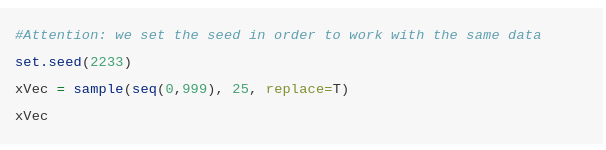
\includegraphics[width=0.8\linewidth,]{img/lab1-exerc2-2-1} \end{center}

\textbf{Resp.:}

\begin{Shaded}
\begin{Highlighting}[]
\FunctionTok{set.seed}\NormalTok{(}\DecValTok{2233}\NormalTok{)}
\NormalTok{xVec }\OtherTok{\textless{}{-}} \FunctionTok{sample}\NormalTok{(}\FunctionTok{seq}\NormalTok{(}\DecValTok{0}\NormalTok{, }\DecValTok{999}\NormalTok{), }\DecValTok{25}\NormalTok{, }\AttributeTok{replace =} \ConstantTok{TRUE}\NormalTok{)}
\NormalTok{xVec}
\end{Highlighting}
\end{Shaded}

\begin{verbatim}
##  [1] 513 773 693 506 706 208 111 713 816 773 465 661 561 883 871 158 498  91  95
## [20]  94 685 564 833 746 425
\end{verbatim}

\begin{center}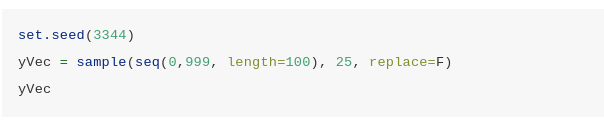
\includegraphics[width=0.8\linewidth,]{img/lab1-exerc2-2-2} \end{center}

\textbf{Resp.:}

\begin{Shaded}
\begin{Highlighting}[]
\FunctionTok{set.seed}\NormalTok{(}\DecValTok{3344}\NormalTok{)}
\NormalTok{yVec }\OtherTok{\textless{}{-}}  \FunctionTok{sample}\NormalTok{(}\FunctionTok{seq}\NormalTok{(}\DecValTok{0}\NormalTok{,}\DecValTok{999}\NormalTok{, }\AttributeTok{length =} \DecValTok{100}\NormalTok{), }\DecValTok{25}\NormalTok{, }\AttributeTok{replace =} \ConstantTok{FALSE}\NormalTok{)}
\NormalTok{yVec}
\end{Highlighting}
\end{Shaded}

\begin{verbatim}
##  [1] 908.18182 888.00000 999.00000  40.36364 433.90909 938.45455 615.54545
##  [8] 898.09091 363.27273 817.36364 736.63636 494.45455 242.18182 948.54545
## [15] 302.72727 181.63636 807.27273 555.00000 353.18182 464.18182 797.18182
## [22] 222.00000 766.90909 988.90909 696.27273
\end{verbatim}

\begin{center}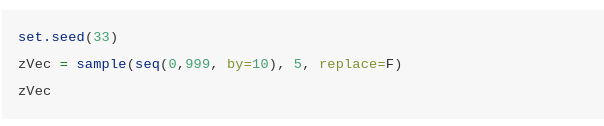
\includegraphics[width=0.8\linewidth,]{img/lab1-exerc2-2-3} \end{center}

\textbf{Resp.:}

\begin{Shaded}
\begin{Highlighting}[]
\FunctionTok{set.seed}\NormalTok{(}\DecValTok{33}\NormalTok{)}
\NormalTok{zVec }\OtherTok{\textless{}{-}}  \FunctionTok{sample}\NormalTok{(}\FunctionTok{seq}\NormalTok{(}\DecValTok{0}\NormalTok{, }\DecValTok{999}\NormalTok{, }\AttributeTok{by=}\DecValTok{10}\NormalTok{), }\DecValTok{5}\NormalTok{, }\AttributeTok{replace =} \ConstantTok{FALSE}\NormalTok{)}
\NormalTok{zVec}
\end{Highlighting}
\end{Shaded}

\begin{verbatim}
## [1] 410  70 850 590  80
\end{verbatim}

\begin{enumerate}
\def\labelenumi{\arabic{enumi}.}
\setcounter{enumi}{2}
\tightlist
\item
  Calcule algumas estatísticas resumidas para os três vetores.
\end{enumerate}

\textbf{Resp.:}

\begin{Shaded}
\begin{Highlighting}[]
\NormalTok{estatisticas }\OtherTok{\textless{}{-}} \ControlFlowTok{function}\NormalTok{(x)\{}
  \FunctionTok{return}\NormalTok{(}
    \FunctionTok{list}\NormalTok{(}
      \StringTok{"length"}\OtherTok{=}\FunctionTok{length}\NormalTok{(x),}
      \StringTok{"mean"}\OtherTok{=}\FunctionTok{mean}\NormalTok{(x),}
      \StringTok{"median"}\OtherTok{=}\FunctionTok{median}\NormalTok{(x),}
      \StringTok{"sd"}\OtherTok{=}\FunctionTok{sd}\NormalTok{(x)}
\NormalTok{    )}
\NormalTok{  )}
\NormalTok{\}}
\end{Highlighting}
\end{Shaded}

\begin{Shaded}
\begin{Highlighting}[]
\FunctionTok{estatisticas}\NormalTok{(xVec)}
\end{Highlighting}
\end{Shaded}

\begin{verbatim}
## $length
## [1] 25
## 
## $mean
## [1] 537.68
## 
## $median
## [1] 564
## 
## $sd
## [1] 267.6224
\end{verbatim}

\begin{Shaded}
\begin{Highlighting}[]
\FunctionTok{estatisticas}\NormalTok{(yVec)}
\end{Highlighting}
\end{Shaded}

\begin{verbatim}
## $length
## [1] 25
## 
## $mean
## [1] 618.3709
## 
## $median
## [1] 696.2727
## 
## $sd
## [1] 289.6566
\end{verbatim}

\begin{Shaded}
\begin{Highlighting}[]
\FunctionTok{estatisticas}\NormalTok{(xVec)}
\end{Highlighting}
\end{Shaded}

\begin{verbatim}
## $length
## [1] 25
## 
## $mean
## [1] 537.68
## 
## $median
## [1] 564
## 
## $sd
## [1] 267.6224
\end{verbatim}

\begin{enumerate}
\def\labelenumi{\arabic{enumi}.}
\setcounter{enumi}{3}
\tightlist
\item
  Selecione os valores em \texttt{yVec} maiores que 600.
\end{enumerate}

\textbf{Resp.:}

\begin{Shaded}
\begin{Highlighting}[]
\NormalTok{yVec[yVec }\SpecialCharTok{\textgreater{}} \DecValTok{600}\NormalTok{]}
\end{Highlighting}
\end{Shaded}

\begin{verbatim}
##  [1] 908.1818 888.0000 999.0000 938.4545 615.5455 898.0909 817.3636 736.6364
##  [9] 948.5455 807.2727 797.1818 766.9091 988.9091 696.2727
\end{verbatim}

\begin{enumerate}
\def\labelenumi{\arabic{enumi}.}
\setcounter{enumi}{4}
\tightlist
\item
  Selecione os valores em \texttt{yVec}que estão entre 600 e 800 e salve-os em um novo valore chamado \texttt{yVec\_sel1}. Escolha os valores em \texttt{yVec}maiores que 600 ou menores que 800 e salve-os em um novo vetor chamado \texttt{yVec\_sel2}. Qual é o comprimento de \texttt{yVec\_sel1} e \texttt{yVec\_sel2}?
\end{enumerate}

\textbf{Resp.:}

\begin{Shaded}
\begin{Highlighting}[]
\NormalTok{yVec\_sel1 }\OtherTok{\textless{}{-}}\NormalTok{ yVec[(yVec }\SpecialCharTok{\textgreater{}} \DecValTok{600}\NormalTok{) }\SpecialCharTok{\&}\NormalTok{ (yVec }\SpecialCharTok{\textless{}} \DecValTok{800}\NormalTok{)]}
\NormalTok{yVec\_sel1}
\end{Highlighting}
\end{Shaded}

\begin{verbatim}
## [1] 615.5455 736.6364 797.1818 766.9091 696.2727
\end{verbatim}

\begin{Shaded}
\begin{Highlighting}[]
\NormalTok{yVec\_sel2 }\OtherTok{\textless{}{-}}\NormalTok{ yVec[(yVec }\SpecialCharTok{\textgreater{}} \DecValTok{600}\NormalTok{) }\SpecialCharTok{|}\NormalTok{ (yVec }\SpecialCharTok{\textless{}} \DecValTok{800}\NormalTok{)]}
\NormalTok{yVec\_sel2}
\end{Highlighting}
\end{Shaded}

\begin{verbatim}
##  [1] 908.18182 888.00000 999.00000  40.36364 433.90909 938.45455 615.54545
##  [8] 898.09091 363.27273 817.36364 736.63636 494.45455 242.18182 948.54545
## [15] 302.72727 181.63636 807.27273 555.00000 353.18182 464.18182 797.18182
## [22] 222.00000 766.90909 988.90909 696.27273
\end{verbatim}

\begin{Shaded}
\begin{Highlighting}[]
\FunctionTok{length}\NormalTok{(yVec\_sel1)}
\end{Highlighting}
\end{Shaded}

\begin{verbatim}
## [1] 5
\end{verbatim}

\begin{Shaded}
\begin{Highlighting}[]
\FunctionTok{length}\NormalTok{(yVec\_sel2)}
\end{Highlighting}
\end{Shaded}

\begin{verbatim}
## [1] 25
\end{verbatim}

\begin{enumerate}
\def\labelenumi{\arabic{enumi}.}
\setcounter{enumi}{5}
\tightlist
\item
  Quais são os valores em \texttt{xVec} que correspondem aos valores em \texttt{yVec} que são maiores que 600? (Por correspondência, dizemos que eles têm as mesmas posições).
\end{enumerate}

\textbf{Resp.:}

\begin{Shaded}
\begin{Highlighting}[]
\NormalTok{xVec[}\FunctionTok{which}\NormalTok{(yVec }\SpecialCharTok{\textgreater{}} \DecValTok{600}\NormalTok{)]}
\end{Highlighting}
\end{Shaded}

\begin{verbatim}
##  [1] 513 773 693 208 111 713 773 465 883 498 685 833 746 425
\end{verbatim}

\begin{enumerate}
\def\labelenumi{\arabic{enumi}.}
\setcounter{enumi}{6}
\tightlist
\item
  Calcule a soma e a diferença dos 5 primeiros elementos dos 2 vetores. Dica: para indexar os 5 primeiros elementos, use \texttt{1:5}.
\end{enumerate}

\textbf{Resp.:}

\begin{Shaded}
\begin{Highlighting}[]
\NormalTok{xVec[}\DecValTok{1}\SpecialCharTok{:}\DecValTok{5}\NormalTok{] }\SpecialCharTok{+}\NormalTok{ yVec[}\DecValTok{1}\SpecialCharTok{:}\DecValTok{5}\NormalTok{]}
\end{Highlighting}
\end{Shaded}

\begin{verbatim}
## [1] 1421.1818 1661.0000 1692.0000  546.3636 1139.9091
\end{verbatim}

\begin{Shaded}
\begin{Highlighting}[]
\NormalTok{xVec[}\DecValTok{1}\SpecialCharTok{:}\DecValTok{5}\NormalTok{] }\SpecialCharTok{{-}}\NormalTok{ yVec[}\DecValTok{1}\SpecialCharTok{:}\DecValTok{5}\NormalTok{]}
\end{Highlighting}
\end{Shaded}

\begin{verbatim}
## [1] -395.1818 -115.0000 -306.0000  465.6364  272.0909
\end{verbatim}

\begin{enumerate}
\def\labelenumi{\arabic{enumi}.}
\setcounter{enumi}{7}
\tightlist
\item
  Para \texttt{xVec} calcule a seguinte fórmula \(\dfrac{\sum_ {i = 1}^n \left(x_i - \bar{x}\right)^2}{n}\), onde \(n\) é o comprimento do vetor e \(\bar{x}\) é a média do vetor. O resultado é igual ao obtido com \texttt{var}? Por quê?
\end{enumerate}

\textbf{Resp.:}

\begin{Shaded}
\begin{Highlighting}[]
\NormalTok{xVar }\OtherTok{\textless{}{-}} \FunctionTok{sum}\NormalTok{((xVec }\SpecialCharTok{{-}} \FunctionTok{mean}\NormalTok{(xVec))}\SpecialCharTok{\^{}}\DecValTok{2}\NormalTok{)}\SpecialCharTok{/}\FunctionTok{length}\NormalTok{(xVec)}
\NormalTok{xVar}
\end{Highlighting}
\end{Shaded}

\begin{verbatim}
## [1] 68756.86
\end{verbatim}

\begin{Shaded}
\begin{Highlighting}[]
\NormalTok{xVar2 }\OtherTok{\textless{}{-}} \FunctionTok{var}\NormalTok{(xVec)}
\NormalTok{xVar2}
\end{Highlighting}
\end{Shaded}

\begin{verbatim}
## [1] 71621.73
\end{verbatim}

A fórmula dada no enunciado do problema calcula a variância populacional enquanto a função \texttt{var} do base R calcula a variância amostral. A diferença entre as duas expressões é que para a variáncia amostral o denominador da fração é igual a \(n - 1\) e não \(n\).

\begin{enumerate}
\def\labelenumi{\arabic{enumi}.}
\setcounter{enumi}{8}
\tightlist
\item
  Para \texttt{xVec}calcule a seguinte fórmula \(\dfrac{\sum_{i=1}^n |x_i - Me| }{n}\), onde \(n\) é o comprimento do vetor e \(Me\) é a mediana do vetor.
\end{enumerate}

\textbf{Resp.:}

\begin{Shaded}
\begin{Highlighting}[]
\FunctionTok{sum}\NormalTok{(}\FunctionTok{abs}\NormalTok{(xVec }\SpecialCharTok{{-}} \FunctionTok{median}\NormalTok{(xVec)))}\SpecialCharTok{/}\FunctionTok{length}\NormalTok{(xVec)}
\end{Highlighting}
\end{Shaded}

\begin{verbatim}
## [1] 217.12
\end{verbatim}

\hypertarget{exercuxedcio-3}{%
\subsubsection{Exercício 3}\label{exercuxedcio-3}}

Considere o seguinte modelo \[Y = \beta_0 + \beta_1 X + \varepsilon\]

onde \(\beta_0 = 2\), \(\beta_1 = 0,3\) e \(\varepsilon\) é uma distribuição normal com média 0 e variância 1.

\begin{enumerate}
\def\labelenumi{\arabic{enumi}.}
\tightlist
\item
  Considerando uma sequência de valores para \(X\) entre 0 e 10, simule 200 valores para \(Y\).
\end{enumerate}

\textbf{Resp.:}

\begin{Shaded}
\begin{Highlighting}[]
\NormalTok{beta\_0 }\OtherTok{\textless{}{-}} \DecValTok{2}
\NormalTok{beta\_1 }\OtherTok{\textless{}{-}} \FloatTok{0.3}

\NormalTok{X }\OtherTok{\textless{}{-}} \FunctionTok{seq}\NormalTok{(}\AttributeTok{from=}\DecValTok{0}\NormalTok{, }\AttributeTok{to=}\DecValTok{10}\NormalTok{, }\AttributeTok{length=}\DecValTok{201}\NormalTok{)}
\NormalTok{eps }\OtherTok{\textless{}{-}} \FunctionTok{rnorm}\NormalTok{(}\DecValTok{201}\NormalTok{, }\AttributeTok{mean =} \DecValTok{0}\NormalTok{, }\AttributeTok{sd =} \DecValTok{1}\NormalTok{)}
\NormalTok{Y }\OtherTok{\textless{}{-}}\NormalTok{ beta\_0 }\SpecialCharTok{+}\NormalTok{ beta\_1 }\SpecialCharTok{*}\NormalTok{ X}
\end{Highlighting}
\end{Shaded}

\begin{enumerate}
\def\labelenumi{\arabic{enumi}.}
\setcounter{enumi}{1}
\tightlist
\item
  Traçar os valores simulados.
\end{enumerate}

\textbf{Resp.:}

\begin{Shaded}
\begin{Highlighting}[]
\NormalTok{df }\OtherTok{\textless{}{-}} \FunctionTok{data.frame}\NormalTok{(X, Y, eps)}

\NormalTok{df }\SpecialCharTok{\%\textgreater{}\%}
  \FunctionTok{ggplot}\NormalTok{() }\SpecialCharTok{+}
    \FunctionTok{geom\_line}\NormalTok{(}\FunctionTok{aes}\NormalTok{(}\AttributeTok{x=}\NormalTok{X, }\AttributeTok{y=}\NormalTok{Y), }\AttributeTok{colour=}\StringTok{"blue"}\NormalTok{)}\SpecialCharTok{+}
    \FunctionTok{geom\_point}\NormalTok{(}\FunctionTok{aes}\NormalTok{(}\AttributeTok{x=}\NormalTok{X, }\AttributeTok{y=}\NormalTok{Y}\SpecialCharTok{+}\NormalTok{eps)) }\SpecialCharTok{+}
    \FunctionTok{theme\_bw}\NormalTok{()}
\end{Highlighting}
\end{Shaded}

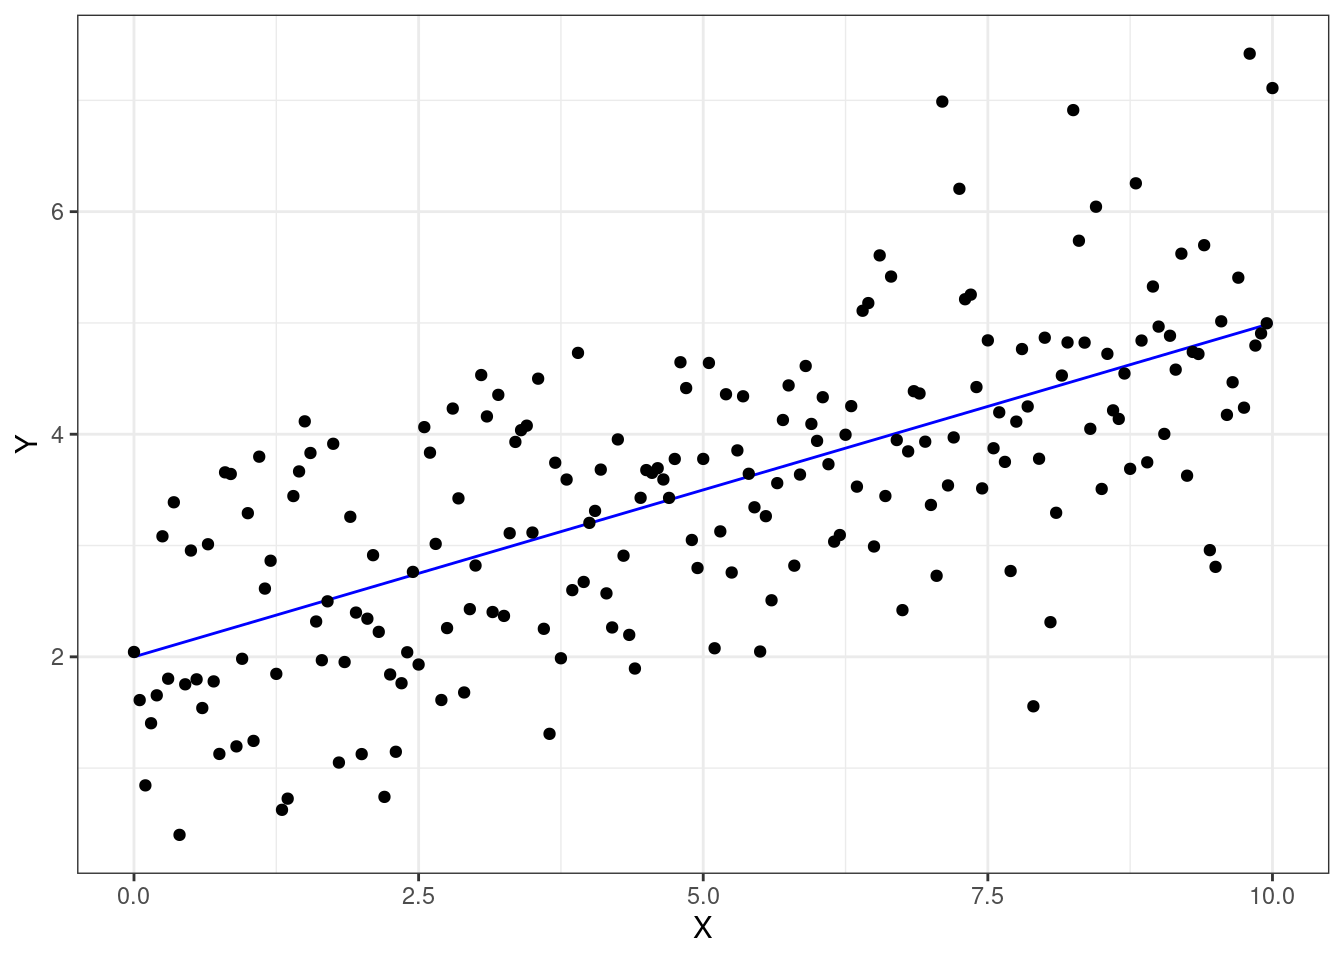
\includegraphics{main_files/figure-latex/unnamed-chunk-26-1}

\hypertarget{a-caucus-race-and-a-long-tale}{%
\section{A caucus-race and a long tale}\label{a-caucus-race-and-a-long-tale}}

\end{document}
